
The first step of developing the game was choosing a programming language that would be helpful in both showing graphics on screen and implement an AI algorithm. The only option that was convenient enough was python as:

\begin{enumerate}
	\item The most famous programming language with AI libraries that have a good documentation.
	\item It is OOP, which means I can have a class for each component of the game easily to make an instance for the AI to train from.
	\item A library to draw graphic on screen while it won't need heavy CPU usage that won't throttle the process of AI learning 
\end{enumerate}

Choosing a library for the game was the first step as it would define the characteristics. I went for \textbf{PyGame} because it was nearly the only one that is good enough with documentation to start with, and quit enough, the main focus isn't about making a game that will have that much of physics in it and 3d animation. For now, the imagined picture of the game is a rectangle as a screen that will have two main component of the game, a wave that is on one side of the screen vertically and one on the other side with the only difference is 350px (the starting amplitude is 50px and the screen width is 400px) and a ball that the \textbf{only purpose for it is to survive as much as it can, without hitting any of the sides of the wave}.\\


I'm minimalist when it comes to developing things, like there wouldn't be splash screen all over, and hard controls, not even hard rules, and it will be the approach I'm following with the game, to break it into steps:

\begin{enumerate}
	\item The accent colour of the game will be black as a background
	\item White will be used to show elements 
	\item Score counter on top
	  \begin{enumerate}
		\item AI mode: show generation and genome number
		\item AI mode: show total runtime
		\item AI mode: show the vision of the ball
	\end{enumerate}
\end{enumerate}

During the writing here, I will raise some questions that might come to your mind while working on some parts (as they might have came to me too) and will try to answer them at the end of every section in the chapter.

\section{Develop the game}\label{develop-the-game}

The files layout of the game will be an \inlineCode{AI.py} file in the root folder, then subfolder named \inlineCode{SurviveLine} with 3 files in it \inlineCode{ballFunc.py}, \inlineCode{waveFunc.py} and \inlineCode{game.py}. To make it easy to make instance of the game, will create a file named \inlineCode{\_\_init\_\_.py} that will only have one line it it \inlineCode{from .game import Game} that means we will have a \inlineCode{Class Game():} in the \inlineCode{game.py} and it is used to call the \inlineCode{game} function as a library in the \inlineCode{AI.py} file (as it is in another folder) and make instance from it. Every major component will have its own class in file to refer later. 

\subsection{Wave functionality}\label{wave-functionality}
To get the base function of wave, there would be a lot of functions to cover like:

\begin{minted}{python}
def draw(self, Display):
	#increase the FPS of game
def changeSpeed(self):
	#change the wave aplitude and increase the wave gap
def changeWave(self):
	#generate a new point on Y axis
def generateWave(self):
	#add point to the list of points
def addPoint(self, index, point):
	#check if there is a gap 
def checkGap(self):
	#function to fill it
def fillGap(self, gap, gapDirection):
	#reset all the self. variable that are made in __init__ class 
def reset(self):
\end{minted}

most of them are self explanatory, but the ones that need more dive into details are the \inlineCode{generateWave}, \inlineCode{checkGap} and \inlineCode{fillGap}.

\subsubsection{Generate wave}


The starting point of the game, in the \inlineCode{waveFunc.py} to make a main class \inlineCode{Class Wave():} with an equation that can generate a wave and at the same time I can change in the variables of the wave to make it harder for the player. These variable are wave amplitude\footnote{is the maximum or lowest height the wave can go in one point to up or down.} or wave frequency\footnote{a number of waves that can go through a fixed distance in amount of time.}.

With all of this in calculation which means that I can make the game harder by making the behaviour unexpected for the next move, also to go extra step, there will be a decrease in the gap between the two waves to limit the player's movement.

\begin{minted}{python}
pointsList_XCord = int((self.HDisplay/2) + self.WaveAmplitude* math.sin(self.waveFreq * ((float(0)/-self.WDisplay)*(2*math.pi) + (time.time()))))
\end{minted}
as you can see, there are some variables that have the \inlineCode{self.} before, that are defined as:

\begin{listing}[!ht]
\begin{minted}{python}
	def __init__(self, wDisplay, hDisplay):
		self.WDisplay = wDisplay
		self.HDisplay = hDisplay
		self.ScoreCount = 0  
		self.waveFreq = 1  # changes difficulty part
		self.WaveGap = 0
		self.GameSpeed = 2  # to increment the difference in time to speed the FPS
		self.FPS = 60
		self.WaveAmplitude = 50
		self.PointsI = 0  # index to loop inside the points list
		self.PointsList = [0]*800
\end{minted}
\caption{the self variable in waveFunc file.}
\label{code:waveFunc self}
\end{listing}


These are the variables that are only (and not specifically) linked to the wave functions, and this is where an important functionality of OOP comes in. Encapsulation is the OOP functionality which means to get all the related data to a class (which is wave class at this point), if it is needed in other classes, then an instance of class wave can be made then the new variable can be used from it.

The equation in figure \ref{code:waveFunc self}  is going to store the X axis coordinates in a list called \inlineCode{PointsList} for the sake of adding points to it once they are generated and show them on screen one by one as if it is loading, because if there isn't a list, then the wave would be a steady visual sine wave (without changing amplitude or frequency yet), this part of code is placed in \inlineCode{def generateWave(self)} function.

There have to be more condition to make the points be generated without disorder, like one point won't be in the other half of screen, which means that when the 350px is added to it, it will be out of the borders of the display.


\subsubsection{Check gap}
After generating a point, with the change in amplitude, the next point that is added to list of points doesn't have a difference of only 1px with the one before it, so it means that there will be a different line segments in the list and a gap between the old point and the new one. To overcome this, after a point is generated, there is a \inlineCode{for loop} that checks if there is only one pixel gap between it (the new point) and the point before it, either it is minus or negative as the gap can be to left or right side.

\begin{figure}[H]
	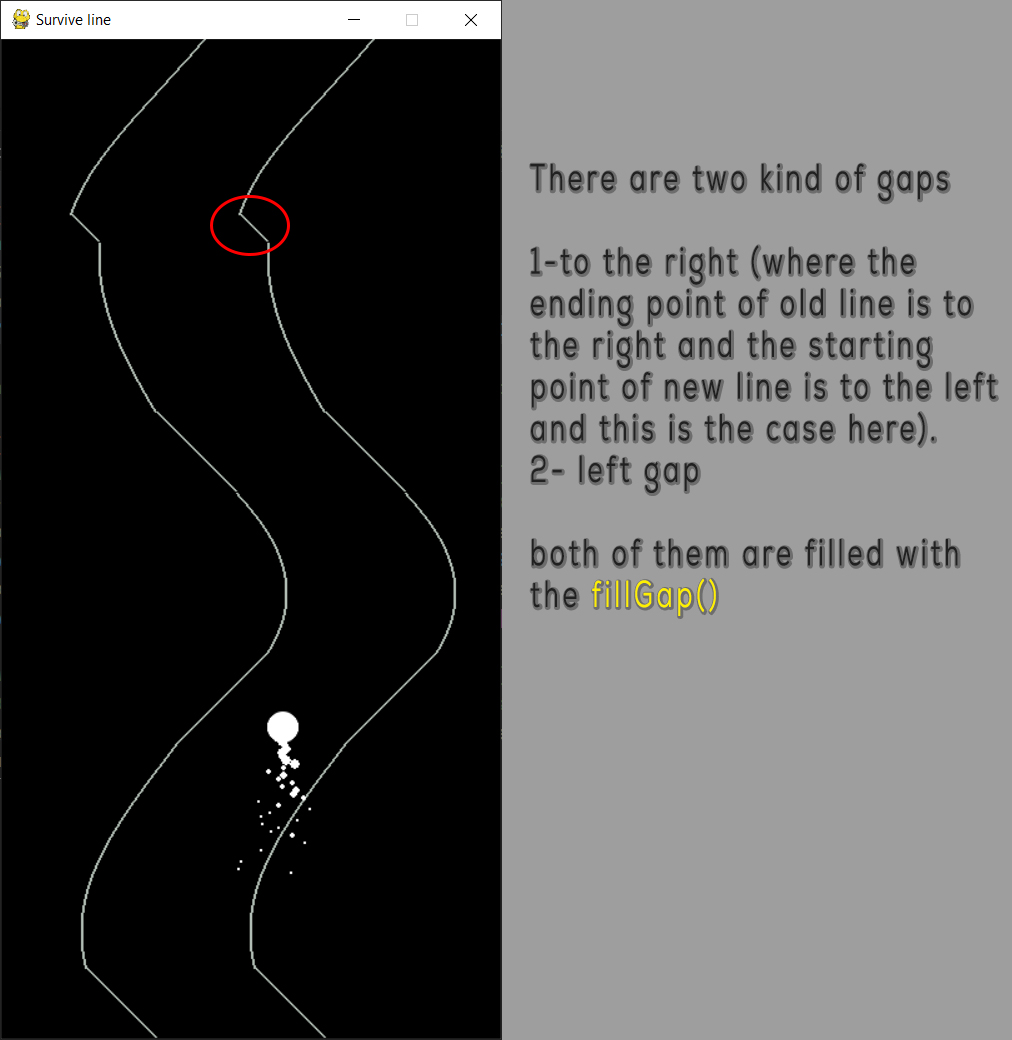
\includegraphics[scale=0.5]{filledGap}
\end{figure}

\subsubsection{Fill gap}
If there is one part which took the most in developing, I would say it is this part, because there were different approaches to solve the problem. First one is either to move the point on y-axis by the gap then make a straight line from the old line segment to it, and the second one was to get the point just to be minus on the x-axis then be linked to it. The first option was better for the sake of visibility and not effecting the next point respectively. There were lots of ways (or you can say conditions) that needs to be covered in the point list, for example what if the gap is at the end of list?  will throw "out of index error" when trying to shift the new point by the amount of gap. One way to cover this is by removing amount of points from the start of the list, then add the same amount at the end where you need it.

Say that the gap is over the limit of list (800Px), dealing with it before was just to make the gap limited to the end of list, so if the point is at index 797 and the gap is 10 (that means there will be an "out of index" error at extra index 6) so it was just to make it limited to  \inlineCode{gap = DISPLAY\_H - POINTS\_I - 1} but the problem is that it wouldn't work on high scale when the amplitude gets higher.
To deal with it is to remove the over-points in gap from the beginning of the list and add empty points of the same amount at the end then make the index go back to the new index, (back to the same example). It will remove 6 points from the beginning of list then add empty 6 points to the end, and shift the index to 6 points in the back so it stays with the new point.

\begin{listing}[H]
\begin{minted}{python}
if self.PointsI + (gap) >= self.HDisplay-1:
	untilEnd = self.HDisplay-self.PointsI
	toAddFromStart = abs(gap-untilEnd)
	del self.PointsList[:toAddFromStart]
	toAdd = [0]*toAddFromStart
	self.PointsList.extend(toAdd)
	self.PointsI -= toAddFromStart
	gap -= 1
\end{minted}
\end{listing}

with every line here looking weirdly by itself, you would need some explanation:

\begin{itemize}
	\item Line 2: calculates the difference between the ending point of list and the starting point of gap.
	\item Line 3: get the difference in gap and the point.
	\item Line 4: delete the amount of point from the beginning of list.
	\item Line 5: create empty list with the amount of delete points from beginning of list.
\end{itemize}

Now with the condition being fulfilled, it comes to fill the gap itself. There would be two options, if the gap is negative or positive, but I will discuss the negative gap and the other one have the same implementation with the difference being the sign.

\begin{listing}[H]
	\begin{minted}{python}
if (gapDirection):
# to move the point according to gap
	self.PointsList[self.PointsI + gap] = self.PointsList[self.PointsI]
	self.PointsList[self.PointsI] = 0
	#the step is different for gap direction, as it would be -1 or +1
	for x in range(self.PointsList[self.PointsI-1], self.PointsList[self.PointsI+gap]-1, (gap//gap)):
		self.PointsList[insideY] = x+1
		if insideY < 799:
			insideY += 1
	\end{minted}
\end{listing}

First it moves the first point in the new line segment by the amount of gap, then resets the old value of it to zero (as it will be part in the straight line). Secondly is a for loop to fill the points incrementally starting from the last point in the old line segment to the new point.

\subsubsection{ Second way to fill the gap}

Fill the gap was basically working on the base of shifting the point on Y-axis, but there might be another approach to tackle this ( the second way I talked about in fixing the problem of gap).

Thinking that it will take more effort to move the point in new line segment in the position that corresponds to the gap, then make a line between the old line segment and the new one. That is a lot to think about, there can be a different way. What if we change the point on x-axis? just to make it close to the old one, I know it is a bit of cheating, but as long as it works, then it is good.

The idea is that, if I can calculate the gap (which I already know) then decrease the new point by the amount of gap + 1 (if it is a positive gap) and will be -1 if it is a negative gap, you may ask, "why didn't you use absolute value for amount of gap as left is the same as right?" because then this would mean that the wave would increment in one way which depends if it is +1 or -1.

The newly implemented function is called \inlineCode{def shiftOnXAxis(self, newPoint)} in \inlineCode{waveFunc.py}.


\subsection{Ball functionality}\label{ball-functionality}
The main focus when working on the ball was to make it as simple as it can be, so a new instance can be done from it without the need to store a self-genome variable, and every genome would have its own variables that can be changed with a new instance made.

\subsubsection{Draw ball}\label{draw-ball}
As the game is based on a \textbf{ball} that survives a line, then I need to display a ball and not a circle (google the difference). There isn't a function to draw a filled ball in one line, so I have to draw an empty circle then fill it. The function \inlineCode{pygame.gfxdraw.aacircle} will draw an anti-aliased circle and \inlineCode{pygame.gfxdraw.filled{\_}circle} draw a filled circle inside of it, then draw a fake rectangle around them with \inlineCode{pygame.Rect} that will deal with the collision (will discuss it in the display game section).

\subsubsection{Generate particles}\label{generate-particles}
This part is little on logic than the other because it was made for the visuality of the game, no output coming out of it to make the game faster or improve something, but it would add a little bit of a characteristic to the game and the vision I have for it.

The particles are made to be in the position of the ball and generate as a way to look like a combustion engine steam coming out ot it, so there are three things to notice here.
\begin{itemize}
\item Location: where the particles will start and their ending point.
\item Velocity: the amount of particles that will be generated in a second.
\item Time: how long they will last on the screen.
\end{itemize}

With this in consideration, we can start writing a function for it 

\begin{listing}[H]
	\begin{minted}{python}
def generateParticles(self):
	Loc =[self.ballCordX, self.ballCordY] 
	Vel = [random.randint(0, 20) / 10 - 1, -3]
	Timer = random.randint(4, 6)
	self.Particles.append([Loc, Vel, Timer])
	for particle in self.Particles:
		particle[0][0] -= particle[1][0]
		particle[0][1] -= particle[1][1]
		particle[2] -= 0.1
		
		pygame.draw.circle(self.GameDisplay, (255, 255, 255), [int(particle[0][0]), int(particle[0][1])], int(particle[2]))
		if particle[2] <= 0:
			self.Particles.remove(particle)
	\end{minted}
\end{listing}

In the \inlineCode{Vel} variable deceleration part, it makes sure that the value we would get, would be a random number between {-1, 1}. The \inlineCode{Timer} to give chaos to the particles so not all of them are released at the same time.

The code would add to the list of particles a new particle with these random starting values, then the \inlineCode{for loop} process each value on its own.

\begin{itemize}
\item Line 7: it process the position on X-axis to the velocity also on the X-axis, same would happen to the Y-coordinates.
\item \inlineCode{particles[2]} is to reduce the particle radius by 0.1 in every frame (which is every loop then).
\item If condition at the end to remove the particle from the list so it wouldn't take much of space with more runtime.
\end{itemize}

This function is possible thanks to [Particles - Pygame Tutorial - YouTube](https://www.youtube.com/watch?v=F69-t33e8tk)

\section{Display the game}\label{display-the-game}




\section{Create AI}\label{create-ai}

\subsection{101 AI}\label{101-ai}


\subsection{What is N.E.A.T?}\label{what-is-neat}

 
\subsection{Tweak AI}\label{tweak-ai}

\subsection{Observation}\label{Observation}

\subsection{Explain the log}\label{explain-the-log]}
 
 
 
 
 
 
 
 
 
 
 
